\section{Vectors, Spans and Bases in $\FR^2$, $\FR^3$ and $\FR^n$.}

    \subsection{Vectors in $\FR^2$}
	We briefly recall some facts about vectors in $\FR^2$. Intuitively, a \textit{vector} of $\FR^2$ can be thought as an arrow encoding a length and a direction. A vector however does not have an origin, so one may draw many arrows in the plane corresponding to the same vector:
	
	\begin{equation*}
	\begin{picture}(70,70)
	\put(0.0,8.0){\line(1,0){70}}
	\put(8.0,0.0){\line(0,1){70}}
	\put(8.0,8.0){\vector(2,1){50}}
	\put(58.0,15.0){\vector(2,1){50}}
	\put(22.0,40.0){\vector(2,1){50}}
	%\put(2.0,0.0){\makebox(0,0)[c]{$\nv$}}
	\put(33.0,10.0){\line(0,-1){4}}
	\put(58.0,10.0){\line(0,-1){4}}
	\put(6.0,33.0){\line(1,0){4}}
	\put(6.0,58.0){\line(1,0){4}}
	%\put(0.0,33.0){\makebox(0,0)[c]{$v_2$}}
	%\put(58.0,0.0){\makebox(0,0)[c]{$v_1$}}
	\end{picture}
	\end{equation*}
	
	One may identify the set of all vectors in $\FR^2$ with the set of points of the plane $\FR^2$, by associating to each point of the plane the vector from the origin to that point. Under this identification, the origin corresponds to a vector called the \textit{null vector} and denoted $\nv$. 

    \begin{df}{}
	Each point and thus each vector $\vv\in\FR^2$ can be denoted by a pair of real numbers (thus the notation $\FR^2$): the horizontal displacement and the vertical displacement. Such a vector is denoted  by the $2 \times 1$ matrix
	\begin{equation*}
	\vv=\vectt{v_1}{v_2}~.
	\end{equation*}
	
	
	\begin{equation*}
	\begin{picture}(70,70)
	\put(0.0,8.0){\line(1,0){70}}
	\put(8.0,0.0){\line(0,1){70}}
	\put(8.0,8.0){\vector(2,1){50}}
	%\put(2.0,0.0){\makebox(0,0)[c]{$\nv$}}
	\put(33.0,10.0){\line(0,-1){4}}
	\put(58.0,10.0){\line(0,-1){4}}
	\put(6.0,33.0){\line(1,0){4}}
	\put(6.0,58.0){\line(1,0){4}}
	\put(0.0,33.0){\makebox(0,0)[c]{$v_2$}}
	\put(58.0,0.0){\makebox(0,0)[c]{$v_1$}}
	\end{picture}
	\end{equation*}
	
	
	It is a very useful convention to write vectors vertically, i.e. as $2 \times 1$ matrices. For typesetting reasons however, we often write that vector as $\vv=(v_1,v_2)^T$, i.e. as a $1\times 2$ matrix instead. 
	\end{df}
	
	We have the following rules for adding two vectors $\vv=(v_1,v_2)^T$ and $\wv=(w_1,w_2)^T$ and for multiplying a vector by a number $\lambda\in \FR$ (called a \textit{scalar}):
	\begin{equation*}
	\vv+\wv=\vectt{v_1}{v_2}+\vectt{w_1}{w_2}:=\vectt{v_1+w_1}{v_2+w_2}\eand \lambda \vv:=\vectt{\lambda v_1}{\lambda v_2}~.
	\end{equation*}
	\begin{equation*}
	\begin{picture}(200,150)(0,50)
	\put(0.0,100.0){\line(1,0){200}}
	\put(100.0,50.0){\line(0,1){150}}
	\put(100.0,100.0){\vector(1,3){30}}
	\put(100.0,100.0){\vector(3,-1){45}}
	\put(100.0,100.0){\vector(-3,1){90}}
	\put(130.0,190.0){\vector(3,-1){45}}
	\put(100.0,100.0){\vector(1,1){75}}
	\put(95.0,92.0){\makebox(0,0)[c]{$\nv$}}
	\put(120.0,180.0){\makebox(0,0)[c]{$\vv_1$}}
	\put(185.0,160.0){\makebox(0,0)[c]{$\vv_1+\vv_2$}}
	\put(140.0,80.0){\makebox(0,0)[c]{$\vv_2$}}
	\put(30.0,130.0){\makebox(0,0)[c]{$-2\vv_2$}}
	\end{picture}
	\end{equation*}
	
	With our convention, the null vector is the vector with coordinates $(0,0)^T$. Note that if we multiply a vector by  $0$, we obtain the null vector: $0\vv=\nv$ for all $\vv\in\FR^2$.
	
%	\paragraph{Scalar product and norm.} We mentioned that a vector in $\FR^2$ encodes a notion of length. We now make this precise. We introduce the  \textit{scalar product} (or  \textit{Euclidean inner product}) $\langle\cdot,\cdot\rangle:\FR^2\times \FR^2\rightarrow\FR$ defined as
%	\begin{equation*}
%	\langle\vectt{u_1}{u_2}, \vectt{v_1}{v_2}\rangle:=u_1v_1+u_2v_2~.
%	\end{equation*}
%	If we take the inner product of a vector $\vv$ with itself, $\langle \vv,\vv \rangle$, we obtain the square of the length\footnote{To see this, draw a picture, insert the coordinates of the vector $\vv$ and use Pythagoras' theorem.} of this vector. We call the length of a vector its \textit{norm} and define
%	\begin{equation*}
%	||\vv||:=\sqrt{\langle \vv,\vv\rangle}~.
%	\end{equation*}
	
	
	
%	\paragraph{Angles.} For parallel vectors $\vv,\wv\in\FR^2$, we have the formula $\langle \vv,\wv\rangle=||\vv||\cdot||\wv||$. More generally we have: 
%%	 and the above lemma states that for perpendicular vectors $\vv,\wv$, it is $\langle \vv,\wv\rangle=0$. These are extreme cases of the general formula
%\begin{prop} For vectors $\uv, \vv $ of $\FR^2$, we have
%	\begin{equation*}
%	\langle \vv,\wv\rangle=||\vv||\cdot||\wv||\cos(\vv,\wv)~,
%	\end{equation*}
%	where $\cos(\vv,\wv)$ denotes the cosine of the angle between $\vv$ and $\wv$.
%	\end{prop}
%%	where $\cos(\vv,\wv)$ denotes the cosine of the angle between $\vv$ and $\wv$. 
%\begin{proof} Uusing coordinates, one gets 
%	\begin{equation*}\label{eq:PythagorasR2}
%	||\vv - \wv||^2 = v_1^2+v_2^2-2v_1w_1-2v_2w_2+w_1^2+w_2^2=||\vv||^2 + ||\wv||^2 -2\langle \vv,\wv\rangle~.
%	\end{equation*}
%	We also know from the law of cosines that, given the triangle spanned by $\vv$ and $\wv$, with sides $||\vv||$, $||\wv||$, $||\vv - \wv||$ and angle $\theta$ opposing side $||\vv - \wv||$, we have
%	\begin{equation*}
%	||\vv - \wv||^2=||\vv||^2 + ||\wv||^2-2||\vv||.||\wv||\cos(\theta)~
%	\end{equation*}
%and the result follows.
%	\end{proof}
%	
%	\begin{prop} Two vectors are perpendicular if and only if their inner product vanishes.\end{prop}
%	\begin{proof}
%		By Pythagoras' theorem, two vectors $\vv,\wv\in\FR^2$ are perpendicular if and only if we have $||\vv||^2+||\wv||^2=||\vv+\wv||^2$. In coordinates, this is equivalent to
%		\begin{equation*}\label{eq:PythagorasR2}
%		v_1^2+v_2^2+w_1^2+w_2^2=v_1^2+v_2^2+2v_1w_1+2v_2w_2+w_1^2+w_2^2=v_1^2+v_2^2+w_1^2+w_2^2+2\langle \vv,\wv\rangle~.
%		\end{equation*}
%		This is equivalent to  $\langle \vv,\wv\rangle=0$.
%	\end{proof}
	
%	\paragraph{Linear combinations.}\label{p:LinCombR2} We can combine both vector addition and scalar multiplication into expressions like this:
%	\begin{equation*}
%	\uv=\lambda \vv+\kappa \wv~,
%	\end{equation*}
%	where $\uv,\vv,\wv\in\FR^2$ and $\lambda,\kappa\in\FR$. More generally, we can have expressions like
%	\begin{equation*}
%	\uv=\lambda_1\vv_1+\lambda_2\vv_2+\lambda_3\vv_3+\cdots+\lambda_n\vv_n~,
%	\end{equation*}
%	where $\uv,\vv_i\in\FR^2$, $\lambda_i\in \FR$ and $n\in\NN$. Expressions of the form $ \lambda_1\vv_1+\lambda_2\vv_2+\lambda_3\vv_3+\cdots+\lambda_n\vv_n$ are called \textit{linear combinations}. 
%	
%	Linear combinations arise naturally when trying to decompose a given vector by means of simpler ones. Denote by $\ev_1 = (1, 0)^T$ and $\ev_2=(0, 1)^T$  the horizontal and vertical vectors of norm one. A vector $\vv$ with coordinates $(v_1, v_2)^T$ can be written as a linear combination of $\ev_1$ and $\ev_2$ as follows:
%	\begin{equation*}
%	\vv=v_1 \ev_1+v_2\ev_2~.
%	\end{equation*}
%	For example, we have:
%	%$(5,3)^T\in\FR^2$ can be written as a linear combination of the vectors $(1,0)^T$ and $(0,1)^T$: $(5,3)^T=5(1,0)^T+3(0,1)^T$. It cannot be written as a linear combination of $(2,1)^T$ and $(4,2)^T$.
%	
%	\begin{equation*}
%	\vectt{5}{3}=5\vectt{1}{0}+3\vectt{0}{1}~.
%	\end{equation*}
	
%	\paragraph{Collinear vectors in $\FR^2$.} Two vectors $\vv,\wv\in\FR^2$ are called \textit{collinear}, if one is obtained by multiplying the other by a scalar. That is, there is a $\lambda\in\FR$ such that
%	\begin{equation*}
%	\vv=\lambda \wv\eor \wv=\lambda \vv~. 
%	\end{equation*}
%	Informally, this means that they define the same direction. There is a simple way to check whether two vectors of $\FR^2$ are collinear. Namely, two vectors $\vv= (v_1, v_2)^T$ and $\wv=(w_1, w_2)^T$ are collinear if and only if 
%	$$ v_1 w_2 - v_2w_1 =0.$$
%	For instance, the vectors $(5, 7)^T$ and $(7, 10)^T$ are not collinear since $5\times 10 - 7 \times 7 = 1 \neq0$.
	
	%%%%%%% stop here %%%%%%%%%
	
%	%
	%\paragraph{Span and basis.} Every vector in $\FR^2$ can be obtained as a linear combination of the vectors $\ev_1$ and $\ev_2$. That is, these two vectors {\em span} $\FR^2$. In general, the {\em span of a set of vetors} $\{\vv_1,\ldots,\vv_n\}$ is the set of their linear combinations. 
	%
	%Consider now two arbitrary vectors $\vv,\wv$. If $\vv=\wv=\nv$, the span of $\vv$ and $\wv$ is just $\{\nv\}$. If they are parallel and $\vv$ or $\wv$ are non-vanishing, then the span of $\vv$ and $\wv$ is a straight line in $\FR^2$ through the origin $\nv$. Otherwise, by lemma \ref{lem:1.1.5}, any vector can be obtained as a linear combination of $\vv$ and $\wv$ and therefore their span is $\FR^2$.
	%
	%A \textit{basis} of $\FR^2$ is a minimal set of vectors that spans $\FR^2$. The vectors $\ev_1$ and $\ev_2$ introduced in \ref{p:LinCombR2} form a basis of $\FR^2$: their span is $\FR^2$ and we need both vectors to span $\FR^2$. On the other hand, $(\ev_1,\ev_2,\vv)$ is not a basis of $\FR^2$. We could write any vector $\uv$ as the linear combination
	%\begin{equation*}
	% \uv=u_1\ev_1+u_2\ev_2+0\vv
	%\end{equation*}
	%for any vector $\vv\in\FR^2$ and therefore the third vector is superfluous.
	
	%\eolec{1.1}{1.2}
	
	
	
	   \subsection{Vectors in $\FR^3$}
	\begin{df}{}
	Most of the notions introduced on $\FR^2$ straightforwardly extend to $\FR^3$. 
	%\paragraph{Linear combinations in $\FR^3$.}
	A point  in the Euclidean dimensions encodes a vector $\vv\in\FR^3$, i.e.\ an arrow from the origin $\nv$ to that point. We describe the vector $\vv$ by a  $3\times 1$ matrix 
	 $$\vv= \vecttt{v_1}{v_2}{v_3},$$
	 or sometimes as a $1 \times 3$ matrix $\vv=(v_1,v_2,v_3)^T$ for typesetting reasons. 
     \end{df}
     
     
     We can add vectors and multiply them by scalars as before:
	\begin{equation*}
	\vv+\wv=\vecttt{v_1}{v_2}{v_3}+\vecttt{w_1}{w_2}{w_3}=\vecttt{v_1+w_1}{v_2+w_2}{v_3+w_3}\eand \lambda \vv=\vecttt{\lambda v_1}{\lambda v_2}{\lambda v_3}~.
	\end{equation*}
%	Linear combinations of vectors in $\FR^3$ are again expressions of the form
%	\begin{equation*}
%	\lambda  \uv+\kappa \vv+\mu \wv\eor \lambda_1\uv_1+\lambda_2\uv_2+\lambda_3\uv_3+\cdots+\lambda_n\uv_n~, etc.
%	\end{equation*}
%	where $\lambda,\kappa,\mu,\lambda_i\in\FR$, $\vv,\wv,\uv_i\in\FR^3$ and $n\in\NN$.
%	% For example, $(5,3,2)^T\in\FR^3$ is not a linear combination of $(1,0,0)^T$ and $(0,1,0)^T$.
%	For instance, $(5,3,2)^T\in\FR^3$ is a linear combination of $(1,0,0)^T$, $(0,1,0)^T$ and $(0,0,1)^T$:
%	\begin{equation*}
%	\vecttt{5}{3}{2}=5\vecttt{1}{0}{0}+3\vecttt{0}{1}{0}+2\vecttt{0}{0}{1}~.
%	\end{equation*}
	
	 \subsection{Vectors in $\FR^n$}
	The generalisation to $\FR^n$ should now be clear.
	
\begin{df}{}
		We define:
	\begin{equation*}
	\FR^n=\left\{\vecttt{x_1}{\vdots}{x_n}~\Big|~x_i\in\FR~,~~~i=1,\ldots,n\right\}~.
	\end{equation*}
	An element of $\FR^n$ is called a \textit{vector} (of $\FR^n$), and is identified with an $n\times 1$ matrix. 
    \end{df}

    \begin{df}{}
    For vectors $\xv, \yv \in \FR^n$ and a scalar $\lambda \in \FR$, we define the following operations on vectors: 
	\begin{itemize}
	\item addition: $\vecttt{x_1}{\vdots}{x_n}+\vecttt{y_1}{\vdots}{y_n}:=\vecttt{x_1+y_1}{\vdots}{x_n+y_n}$, 
	\item multiplication by a scalar:  $\lambda \vecttt{x_1}{\vdots}{x_n}:=\vecttt{\lambda x_1}{\vdots}{\lambda x_n}.$
	\end{itemize}
\end{df}

From a given family of vectors, one can construct new vectors using additions and multiplication scalars.

\begin{df}{}
	Let $\vv_1, \ldots, \vv_k\in \FR^n$. A \textit{linear combination} of $\vv_1, \ldots, \vv_k$ is a vector of the form 
	$$\lambda_1 \vv_1 + \ldots + \lambda_k \vv_k ~~~~~~ \mbox{ for some } \lambda_1, \ldots, \lambda_k \in \FR.$$ 
\end{df}

\begin{example}
	The vector $\vectt{1}{3}\in \FR^2$ is a linear combination of $\vectt{1}{2}$ and $\vectt{2}{3}$, since
	$$ \vectt{1}{3} = 3\vectt{1}{2} - \vectt{2}{3}.$$
	\end{example}

\begin{exercise}{}
Let 
\[
\vv=\begin{pmatrix}1\\-1\end{pmatrix},
\qquad 
\wv=\begin{pmatrix}-1\\3\end{pmatrix}.
\]
\begin{enumerate}[label=\alph*)]
\item Compute $\vv+\wv$, $\vv-\wv$ and $3\vv-2\wv$.
\item Find all $\lambda\in\FR$ such that $\vv+\lambda\wv=\nv$ (if any).
\item Are $\vv$ and $\wv$ scalar multiples of one another?
\end{enumerate}
\end{exercise}

\begin{solution}{}
\begin{enumerate}[label=\alph*)]
\item 
\[
\vv+\wv=\begin{pmatrix}1-1\\-1+3\end{pmatrix}=\begin{pmatrix}0\\2\end{pmatrix},\qquad
\vv-\wv=\begin{pmatrix}1+1\\-1-3\end{pmatrix}=\begin{pmatrix}2\\-4\end{pmatrix}.
\]
Also
\[
3\vv-2\wv=3\begin{pmatrix}1\\-1\end{pmatrix}-2\begin{pmatrix}-1\\3\end{pmatrix}
=\begin{pmatrix}3\\-3\end{pmatrix}-\begin{pmatrix}-2\\6\end{pmatrix}
=\begin{pmatrix}5\\-9\end{pmatrix}.
\]

\item Solve $\vv+\lambda\wv=\nv$:
\[
\begin{pmatrix}1\\-1\end{pmatrix}+\lambda\begin{pmatrix}-1\\3\end{pmatrix}
=\begin{pmatrix}0\\0\end{pmatrix}
\quad\Longleftrightarrow\quad
\begin{cases}
1-\lambda=0,\\
-1+3\lambda=0.
\end{cases}
\]
The first gives $\lambda=1$ while the second gives $\lambda=\tfrac13$, which is impossible. Hence there is \emph{no} $\lambda$ with $\vv+\lambda\wv=\nv$.

\item If $\vv=\mu\wv$, then $1=-\mu$ and $-1=3\mu$, giving $\mu=-1$ and $\mu=-\tfrac13$, a contradiction. So they are not scalar multiples. This is just rephrasing (b) with $\mu = - \lambda$.
\end{enumerate}
\end{solution}





Writing a vector as a linear combination of other vectors can be thought of as `decomposing' that vector. Given a family of vectors $\vv_1, \ldots, \vv_k$ of $\FR^n$, we will study the following questions: 
\begin{itemize}
	\item Can every vector of $\FR^n$ be written as a linear combination of $\vv_1, \ldots, \vv_k$?
	\item  If not, \textit{which} vectors of $\FR^n$ can be written as a linear combination of $\vv_1, \ldots, \vv_k$?
	\item \textit{In how many ways} can a vector of $\FR^n$ be written as a linear combination of $\vv_1, \ldots, \vv_k$?
\end{itemize}

\paragraph{The standard basis of $\FR^n$.} 

There is already a standard family of vectors for which these questions have a simple answer.

\begin{df}{}
	We introduce the following vectors	of $\FR^n$:
	$$\ev_1:= \vectttt{1}{0}{\vdots}{0}, \ev_2 \coloneqq \vectttt{0}{1}{0}{\vdots},\ldots, \ev_n:=\vectttt{0}{\vdots}{0}{1}.$$
	This family of vectors is generally called the \textit{standard basis} of $\FR^n$.
\end{df}

	%\paragraph{Remark.} $\bigstar$ Although it is impossible to imagine a four- or higher-dimensional space, some intuition can be obtained from reading Edwin A. Abott's novel ``Flatland: A Romance of Many Dimensions'' from 1884. The author describes life in a two-dimensional world. As a two-dimensional creature, he also visits a one-dimensional world and encounters a three-dimensional sphere. What would a four-dimensional sphere passing through our three-dimensional world look like?
	
%	For instance, in the case of $\FR^2$, these vectors correspond to the standard unit vectors often denotes $\iv$ and $\jv$.
	
	\begin{thm}{}
		Every vector $\xv = (x_1, \ldots, x_n)^T$ of $\FR^n$ can be written in a unique way as a linear combination of $\ev_1, \ldots, \ev_n$, namely:
		$$\xv = x_1\ev_1 + \ldots + x_n\ev_n.$$
		\end{thm}

\begin{example}
	The vector $\vecttt{1}{3}{5}\in \FR^3$ can be written as a linear combination of the standard basis vectors for $\FR^3$, $\ev_1, \ev_2, \ev_3$ since
	$$ \vecttt{1}{3}{5} = \ev_1 + 3 \ev_2 + 5 \ev_3 =\vecttt{1}{0}{0} +3\vecttt{0}{1}{0} + 5 \vecttt{0}{0}{1}.
    $$
	\end{example}

Note that it is also possible to use a {\it non}-standard basis to describe the vectors, as in the following example.

\begin{example}
	The vector $\vecttt{1}{3}{5}\in \FR^3$ from the previous example can also be written as a linear combination of the non-standard basis vectors for $\FR^3$, $\ev_1, \vec{f}_2, \vec{f}_3$ 
    where
    $$
    \vec{f}_2 = \vecttt{0}{1}{1}, \; \vec{f}_3 = \vecttt{0}{1}{-1}
    $$
    since
	$$ \vecttt{1}{3}{5} = \ev_1 + 4 \vec{f}_2 -1 \vec{f}_3 =\vecttt{1}{0}{0} +4\vecttt{0}{1}{1} - \vecttt{0}{1}{-1}.
    $$
	\end{example}

\begin{exercise}{}
\begin{question}
    Can I use $\vecttt{1}{2}{3}$ along with $\vecttt{1}{0}{0}$ and $\vecttt{0}{1}{0}$ as basis for
     $\FR^3$?
    \end{question}
 \end{exercise}


 
	\subsection{Systems of linear equations in vector form.}
	
%	Before proving this result, we need some notation:
	
	%%%%%%%%%% TO DO: Rewrite this in the simpler form Ax = x_1 Col_1 + ... + x_n Col_n.
	

		Consider a system of linear equations whose associated matrix is an $m\times n$ matrix of the form: 
		$$A:= \left(\begin{array}{cccc}
		a_{11}&a_{12}&\ldots&a_{1n}\\
		a_{21}&a_{22}&\ldots&a_{2n}\\
		\vdots &\vdots &   & \vdots\\
		a_{m 1}&a_{m 2}&\ldots&a_{m n}\\
		\end{array}\right) = \left(\begin{array}{c|c|c} \mathrm{col}_1(A) & \cdots & \mathrm{col}_n(A)
		\end{array}\right) .$$
		For $\xv = \vectttt{x_1}{x_2}{\vdots}{x_n}		$ a vector of $\FR^n$, we define : 
		$$A\xv := x_1 \mathrm{col}_1(A) + \ldots + x_n \mathrm{col}_n(A) \in \FR^n.$$
		In other  words, for $1 \leq i \leq m$, the $i$-th component of $A\xv$ is $(A\xv)_i = \sum_{1 \leq k \leq n} a_{ik}x_k.$
		%	$A\xv:= \vectttt{a_{11}x_1+a_{12}x_2+\ldots+a_{1n}x_n}{a_{21}x_1+a_{22}x_2+\ldots+a_{2n}x_n}{\vdots}{a_{m1}x_1+a_{m2}x_2+\ldots+a_{mn}x_n}\in \FR^n.$




	Consider the following system of linear equations:
	\begin{equation*}
\begin{aligned}
\left\{	\begin{array}{ccc}
a_{11}x_1+a_{12}x_2+\ldots+a_{1n}x_n& = & b_1\\
a_{21}x_1+a_{22}x_2+\ldots+a_{2n}x_n& = & b_2\\
\vdots & & \vdots\\
a_{m1}x_1+a_{m2}x_2+\ldots+a_{mn}x_n& = & b_m
\end{array}\right.
%~~~\rightsquigarrow~~~\\[0.3cm]
%\matrixbig{a}{m}{n}\vectbig{x}{n}=\vectbig{b}{m}~.
%\end{aligned}
%\end{equation*}
%We see that systems of linear equations can be written in matrix form $A\xv=\bv$. Example:
%\begin{equation*}
% \begin{array}{ccc}
%  5 x_1 + 3 x_2 & = & 10\\
% -2 x_1 + 2 x_2 & = & 2
% \end{array}
%~~~\rightsquigarrow~~~\left(
% \begin{array}{cc}
% 5 & 3 \\ -2 & 2
% \end{array}\right)\vectt{x_1}{x_2}=\vectt{10}{2}~.
\end{aligned}
\end{equation*}

Let $A$ be the matrix associated to this system, and let $\yv = \vecttt{y_1}{\vdots}{y_n}\in \FR^n.$ A vector $\xv=\vecttt{x_1}{\vdots}{x_n}$ is solution of that system if and only we have: 
%the following equality between vectors: 
$$A\xv = \yv.$$
Solving that system is thus equivalent to the following problem: 
\begin{center}
	\textit{Is $\yv \in \FR^n$ a linear combination of $\mathrm{col}_1(A), \ldots, \mathrm{col}_n(A)$?}
\end{center}


%In practice, this result means that any equation between vectors can by solving by reducing it to a system of linear equations. This approach will be used many times in this course.
	Thus, a $m \times n$ matrix is not `just a bunch of numbers', but we can use it to associate to a vector $\xv \in \FR^n$ a new vector $A\xv \in \FR^m$. In other words, we can associate to any $m \times n $ matrix a map from $\FR^n$ to $\FR^m$.
	
	\subsection{Spans of vectors and spanning families in $\FR^n$} 
	
Given a family $\vv_1, \ldots, \vv_k$ of vectors of $\FR^n$, we start by considering the questions: What vectors of $\FR^n$ can be obtained as a linear combination of $\vv_1, \ldots, \vv_k$? We first introduce some definition:
	
	\begin{df}{} The  \textit{ span} of a family $\vv_1, \ldots, \vv_k$ of vectors of $\FR^n$ is the set span$(\vv_1, \ldots, \vv_k)$ of vectors of $\FR^n$ that can be written as a linear combination of $\vv_1, \ldots, \vv_k$. In other words,
		$$\mathrm{span}(\vv_1, \ldots, \vv_k) = \{ \sum_{i=1}^k \lambda_i \vv_i ~|~ \lambda_i \in \FR \mbox{  for every } i\}.$$
%		We say that a family $\vv_1, \ldots, \vv_k$ of vectors of $\FR^n$ \textit{spans} $\FR^n$, or that $\FR^n$ is \textit{spanned by}  $\vv_1, \ldots, \vv_k$, if every vector of $\FR^n$ can be written as a linear combination of $\vv_1, \ldots, \vv_k$.
	\end{df}
	
	
	Checking whether a given vector is a linear combination of a family of vectors is checked by solving a system of linear equations. Here is an example: 
	
	\begin{example} Let us determine whether the vector  $(3,-4,2)^T$ is a linear combination of  $(1,0,2)^T$ and $(1,1,3)^T$. We have to solve the equation 
		\begin{equation*}
		\lambda \vecttt{1}{0}{2}+\kappa \vecttt{1}{1}{3}= \vecttt{3}{-4}{2}
		\end{equation*}
		with variables $\lambda, \kappa \in \FR$. Using coordinates, we express this as a system of linear equations, and perform Gaussian elimination: 
		\begin{equation*}\label{rem}
		\begin{aligned}
		\left(\begin{array}{cc|c}
		1 & 1  & 3 \\
		0 & 1 & -4 \\
		2 & 3  & 2
		\end{array}\right)
		\elt{R_3\leftrightarrow R_3-2R_1}
		\left(\begin{array}{cc|c}
		1 & 1  &3 \\
		0 & 1  & -4 \\
		0 & 1  & -4
		\end{array}\right)
		\elt{R_3\rightarrow R_3-R_2}
		\left(\begin{array}{cc|c}
		1 & 1  &3 \\
		0 & 1  & -4  \\
		0 & 0 & 0 
		\end{array}\right)
		\end{aligned}
		\end{equation*}
		%\item The vectors $\vv_1=(1,0,0)^T$, $\vv_2=(0,1,0)^T$ and $\vv_3=(1,1,0)^T$ are linearly dependent, since $1\cdot \vv_1+1\cdot \vv_2-1\cdot \vv_3=\nv$ (and also $2\cdot \vv_1+2\cdot \vv_2-2\cdot \vv_3=\nv$ etc.).\\
		%\item Similarly, the vectors $\vv_1=(3,2,1)^T$ and $\vv_2=(0,0,0)^T$ are linearly dependent, because $0\cdot \vv_1+1\cdot \vv_2=\nv$ (and also $0\cdot \vv_1+2\cdot \vv_2=\nv$).\\
		%\item On the other hand, the vectors $\ev_1=(1,0,0)^T$, $\ev_2=(0,1,0)^T$ and $\ev_3=(0,0,1)^T$ are linearly independent, because $a_1\cdot \ev_1+a_2\cdot \ev_2+a_3\cdot \ev_3=\nv$ implies $a_1=a_2=a_3=0$.
		From this echelon form, we see that the system has exactly one solution (all variables are pivot variables and no inconsistent line). We solve the resulting system by substitution, which yields 
		$\kappa = -4$ and $\lambda = 3 - \kappa = 7$. Thus, 
		\begin{equation*}
		7 \vecttt{1}{0}{2} -4 \vecttt{1}{1}{3}= \vecttt{3}{-4}{2}.
		\end{equation*}
	\end{example}

\begin{exercise}{Linear combination test in $\FR^3$}
Determine whether the vector $\vecttt{2}{5}{1}$ is a linear combination of
$\vecttt{1}{1}{0}$ and $\vecttt{0}{2}{1}$. If it is, find scalars $\lambda,\kappa\in\FR$
such that
\[
\lambda \vecttt{1}{1}{0}+\kappa \vecttt{0}{2}{1}=\vecttt{2}{5}{1}.
\]
\end{exercise}

\begin{solution}{}
We must solve
\[
\lambda \vecttt{1}{1}{0}+\kappa \vecttt{0}{2}{1}=\vecttt{2}{5}{1}.
\]
In coordinates this becomes the linear system
\[
\begin{cases}
\lambda \;=\; 2,\\
\lambda+2\kappa \;=\; 5,\\
\kappa \;=\; 1.
\end{cases}
\]
which is inconsistent.\\

Equivalently, we row-reduce the augmented matrix:
\[
\begin{aligned}
\left(\begin{array}{cc|c}
1 & 0 & 2\\
1 & 2 & 5\\
0 & 1 & 1
\end{array}\right)
\elt{R_2\rightarrow R_2-R_1}
\left(\begin{array}{cc|c}
1 & 0 & 2\\
0 & 2 & 3\\
0 & 1 & 1
\end{array}\right)
\elt{R_2\leftrightarrow R_3}
\left(\begin{array}{cc|c}
1 & 0 & 2\\
0 & 1 & 1\\
0 & 2 & 3
\end{array}\right)
\elt{R_3\rightarrow R_3-2R_2}
\left(\begin{array}{cc|c}
1 & 0 & 2\\
0 & 1 & 1\\
0 & 0 & 1
\end{array}\right).
\end{aligned}
\]
The last row represents $0\lambda+0\kappa=1$, which is impossible. Hence the system
has no solution, so $\vecttt{2}{5}{1}$ is \emph{not} a linear combination of
$\vecttt{1}{1}{0}$ and $\vecttt{0}{2}{1}$.
\end{solution}




	Since checking whether a given vector $\vv$ is a linear combination of vectors $\vv_1, \ldots, \vv_k$  is checked by solving a system of linear equations, it follows  that there is either no way to write $\vv$ as a linear combination $\vv_1, \ldots, \vv_k$ (precisely when $\vv$ is not in the span of $\vv_1, \ldots, \vv_k$), exactly one way or infinitely many ways.

	
	
	\begin{thm}{}
		Let $\uv_1, \ldots, \uv_k$ be a family of vectors of $\FR^n$ and consider $V \coloneqq \mathrm{span}(\uv_1, \ldots, \uv_k)$. We have the following: 
		\begin{itemize}
			\item $\nv \in V$,
			\item For every $\xv, \yv \in V$, we also have $\xv + \yv \in V$.
			\item For every $\xv \in V$ and $\lambda \in \FR$, we also have $\lambda \xv \in V$.
		\end{itemize}
		
		
		More generally, any linear combination of vectors of $V$ is again in $V$.
		\end{thm}
	
	\begin{df}{}
		A subset of $\FR^n$ containing the null vector and stable under linear combinations is called a \textit{subspace} of $\FR^n$.
		\end{df}
	
	
	
 	The algebraic properties of spans of vectors mentioned above have a geometric counterpart: Spans of vectors, seen as subsets of $\FR^n$, have a very simple shape: line or plane through the origin in $\FR^3$ for instance. More complicated shapes, such as spheres, hyperboloids, etc. can never be spans.
	

	As an illustration, we now list the various possibilities for the span of two vectors of $\FR^2$. In particular, we see that such spans are geometrically very simple. 
    
	\begin{thm}
		
		The span of two vectors of $\FR^2$ is either: 
		\begin{itemize}
             \item[]
			\item[(i)] $\{\nv\}$,
			\item[(ii)] a straight line through the origin,
			\item[(iiii)] all of $\FR^2$.
		\end{itemize}	
	\end{thm}
	\begin{proof}Consider two arbitrary vectors $\vv = (v_1, v_2)^T, \wv= (w_1, w_2)^T$. If $\vv=\wv=\nv$, the span of $\vv$ and $\wv$ is just $\{\nv\}$. If they are collinear and for instance $\vv$ is non-vanishing, then the span of $\vv$ and $\wv$ is the straight line parallel to $\vv$ going through the origin. 
		
		If they are not collinear, then we now show that $\vv$ and $\wv$ span $\FR^2$. Let $\uv=(a, b)^T$ be an arbitrary vector of $\FR^2$. We want to write $\uv$ as a linear combination of $\vv$ and $\wv$. In other words, we want to find numbers $\lambda, \mu \in \FR$ such that $\lambda\vv + \mu \wv = \uv$. By taking coordinates, this yields the following equations: 
		\begin{equation*}
		\begin{cases}
		\lambda v_1+\mu w_1 &=u_1\\
		\lambda v_2+\mu w_2 &=u_2
		\end{cases}
		\end{equation*}
		Here, the variables are $\lambda$ and $\mu$, and the coefficients $u_1, u_2, v_1, v_2, w_1, w_2$ are constants. We thus have a system of linear equations. We perform the following row operations: 
		
		\begin{equation*}\label{rem}
		\begin{aligned}
		\melt{R_1\rightarrow w_2R_1-w_1R_2\\ R_2 \rightarrow v_1R_2 - v_2R_1}
		\begin{cases}
		(v_1w_2-v_2w_1)\lambda &=  u_1w_2-u_2w_1  \\
		(v_2w_1-v_1w_2)\mu &= u_2v_1-u_1v_2
		\end{cases}
		\end{aligned}
		\end{equation*}
		Since $\vv$ and $\wv$ are not collinear, we have $v_1w_2-v_2w_1 \neq0$, so we can find solutions $\lambda$ and $\mu$ in terms of the other constants. Thus, there is a solution to our system of equations, so $\uv$ is a linear combination of $\vv$ and $\wv$.
	\end{proof}
	
	%	\paragraph{Remark.} It is not necessary to remember the previous formulas to write a given vector as a linear combination of two given vectors. Instead, when given concrete vectors, use Gaussian elimination to solve the system of linear equations. For instance, try to write the vector $(2, -1)^T$ as a linear combination of $(2, 5)^T$ and $(1, 4)^T$ by solving the associated system of linear equations.
	

	
	\subsection{Spanning families.}
	
	\begin{df}{} 
		We say that a family $\vv_1, \ldots, \vv_k$ of vectors of $\FR^n$ \textit{spans} $\FR^n$ (or is a \textit{spanning family} of $\FR^n$, or that $\FR^n$ is \textit{spanned by}  $\vv_1, \ldots, \vv_k$), if $span (\vv_1, \ldots, \vv_k) = \FR^n$, that is,  if every vector of $\FR^n$ can be written as a linear combination of $\vv_1, \ldots, \vv_k$.
	\end{df}
	
	\begin{thm}{}
    Let $\vv_1, \ldots, \vv_k$ be a spanning family of $\FR^n$. Then $k \geq n$. In other words, a spanning family of $\FR^n$ contains at least $n$ vectors. 
	\end{thm}
	\begin{proof}
		Given a vector $\bv = (b_1, \ldots, b_n)^T$ of $\FR^n$, we have to consider the equation 
		\begin{equation*}
		\lambda_1\vv_1 + \cdots + \lambda_k\vv_k = \bv,
		\end{equation*}
		where $\lambda_1, \ldots, \lambda_k$ are variables. Taking coordinates gives us a system of $n$ equations (one for each coordinate of $\FR^n$) with $k$ variables. We can now perform Gaussian elimination to get a system in echelon form. We will now show that each row contains a pivot, which will be enough to conclude that $k \geq n$: Since each pivot must be strictly to the right of the pivots of the previous rows, this means that there must be at least as many columns as rows in the associated matrix, hence $k \geq n$.
		
		If there was a row without a pivot, then the last row of the augmented matrix the echelon form would be of the form 
		\begin{equation*}
		\begin{aligned}
		\left(\begin{array}{ccc|c}
		0 & \cdots & 0  & \beta 
		\end{array}\right),
		\end{aligned}
		\end{equation*}
		where $\beta$ is a non-trivial linear combination of $b_1, \ldots, b_n$. Note that if $\beta \neq 0$, then we have a forbidden row, and the system has no solution. We can now choose specific values of $b_1, \ldots, b_n$ such that $\beta \neq 0$. 
%		Thus, start from the augmented matrix 
%		\begin{equation*}
%		\begin{aligned}
%		\left(\begin{array}{ccc|c}
%		\times &\cdots & \times & 0\\
%		\vdots &\ddots & \vdots & \vdots\\  
%		0 & \cdots & 0  & 1 
%		\end{array}\right)
%		\end{aligned}
%		\end{equation*}
%		and note that this corresponds to a system with no solution. Now, perform the reverse row operations to end up with an augmented matrix of the form 
%		\begin{equation*}
%		\begin{aligned}
%		\left(\begin{array}{ccc|c}
%		v_{11} &\cdots & v_{1k} & b_1\\
%		\vdots &\ddots & \vdots & \vdots  \\  
%		v_{n1} & \cdots & v_{nk}  & b_n 
%		\end{array}\right)
%		\end{aligned}
%		\end{equation*}
		This corresponds to an equation of the form 
		\begin{equation*}
		\lambda_1\vv_1 + \cdots + \lambda_k\vv_k = \vecttt{b_1}{\vdots}{b_n}
		\end{equation*}
		which also has no solution. Thus, the vector $\bv=(b_1, \ldots, b_n)^T$ is not a linear combination of $\vv_1, \ldots, \vv_n$, hence these vectors do not form a spanning family.
	\end{proof}
	
	
	
	
	
	
	
	\subsection{Linearly independent families in $\FR^n$}
	
	
%	
%	$$  \vv_1 = \vectt{1}{0}, \vv_2=\vectt{0}{1}, \vv_3=\vectt{1}{1}.  $$
%	
%	For instance, the vector $\vv=(1,2)^T$ is in the span of $\vv_1, \vv_2, \vv_3$. Indeed, we have
%
%	$$~~~~~~~~~~~~~~~~~~\vv = \vv_1 + 2\vv_2  ~~~~~~~~~~~~~~~~~~(E_1)$$
%	but notice also that we have for instance
%	$$~~~~~~~~~~~~~~~~~~\vv = \vv_2 + 2\vv_3.  ~~~~~~~~~~~~~~~~~~  (E_2)$$
%	
%	Unlike the case of the standard basis of $\FR^n$, there is no uniqueness in the decomposition of $\vv$ as a linear combination of $\vv_1, \vv_2, \vv_3$. This can be explained by the fact that there is already a relation between $\vv_1, \vv_2, \vv_3$. Indeed, we have 
%	$$\vv_3 = \vv_1 + \vv_2.$$
%and this relation can be used to deduce the equation ($E_1$) from the equation ($E_2$).


We now study family of vectors $\vv_1, \ldots, \vv_k \in \FR^n $ for which there is a unique way to write a given in the span as a linear combination of $\vv_1, \ldots, \vv_k$.

\begin{df}{}
	A family of vectors of $\FR^n$ is \textit{linearly dependent} if one of the vectors is a linear combination of the other vectors. Equivalently, a family of vectors $\vv_1, \ldots, \vv_k$ is linearly dependent if there exist scalars $\lambda_1, \lambda_k\in \FR$ not all zero such that 
	$$\lambda_1 \vv_1 + \ldots + \lambda_k \vv_k = \nv.$$
	
	A family of vectors $\vv_1, \ldots, \vv_k$ is \textit{linearly independent} if for every $\lambda_1, \lambda_k\in \FR$, we have  
	$$\lambda_1 \vv_1 + \ldots + \lambda_k \vv_k = \nv ~~ \Longrightarrow ~~ \lambda_1= \cdots = \lambda_k = 0.$$
	\end{df}
	
%	
%	\begin{example}
%		
%		TBC???
%		\end{example}
%	
	
		A family of vectors $\vv_1, \ldots, \vv_k$  is linearly independent if and only if there is a unique way to write any vector of the span as a linear combination of $\vv_1, \ldots, \vv_k$.
	
	
%	
%	
%	\paragraph{A first look at linear dependence in $\FR^3$.}
%	% If two vectors $\uv,\vv\in\FR^3$ are parallel to each other, i.e.\ one is a multiple of the other, the set of their linear combinations or their span is just $\nv$ if $\uv=\vv=\nv$, and a line through the origin otherwise. If they are not parallel, their linear combinations form a plane containing the null-vector $\nv$. A third vector $\wv$ is an element of this plane, if it can be written as a linear combination of the other two:
%	Given three vectors $\uv, \vv, \wv$, we say that they are \textit{linearly dependent} if one can be written as a linear combination of the other two, for instance
%	\begin{equation*}
%	\wv=\lambda \uv+\kappa\vv~~~~ \mbox{for some } \lambda, \kappa \in \FR.
%	\end{equation*}
%	An equivalent definition, which has the advantage of being symmetric in the vectors $\uv, \vv, \wv$ and thus easier to work with, is that the vectors $\uv,\vv,\wv$ are \textit{linearly dependent} if there is a \textit{non-trivial linear combination} (i.e.\ at least one of the scalars $\lambda,\kappa,\mu$ is not zero) of the form
%	\begin{equation*}
%	\lambda \uv+\kappa \vv+\mu \wv=\nv~~~~ \mbox{for some }  \lambda, \kappa, \mu \in \FR, 
%	\end{equation*}
%	such that at least  one of the scalars $\lambda,\kappa,\mu$ is not zero. Such a linear combination is called a \textit{non-trivial linear combination}.
%	
%	If $\uv, \vv, \wv$ are not linearly dependent, they are called \textit{linearly independent}. This is equivalent to the following implication: 
%	\begin{equation*}
%	\mbox{For every }  \lambda, \kappa, \mu \in \FR, ~~~  \lambda \uv+\kappa \vv+\mu \wv=\nv \Rightarrow   \lambda = \kappa = \mu  = 0. 
%	\end{equation*}
%	Note that linear independence implies that if a vector can be decomposed as a linear combination of linearly independent vectors, then this decomposition is unique. Indeed, if 
%	\begin{equation*}
%	\lambda \uv+\kappa \vv+\mu \wv=\lambda' \uv+\kappa' \vv+\mu' \wv,
%	\end{equation*}
%	then
%	\begin{equation*}
%	(\lambda- \lambda') \uv+(\kappa- \kappa') \vv+(\mu- \mu') \wv=\nv,
%	\end{equation*}
%	which by linear independence implies $\lambda =\lambda', \kappa = \kappa',$ and $\mu = \mu'$.
	
	
 Determining whether vectors are linearly independent amounts to solving a system of linear equations, which we do using Gaussian elimination. 
 
 	\begin{thm}{}
 	    To determine whether vectors $\vv_1,\ldots,\vv_k$ are linearly independent, one uses Gaussian elimination to find all solutions to the system
 	\begin{equation*}
 	c_1\vv_1+c_2\vv_2+\ldots+c_k\vv_k=\nv~.
 	\end{equation*}
 	If all variables $c_1,\ldots, c_k$ are pivot variables, this homogeneous system of linear equations has only the trivial solution $c_1=c_2=\ldots=c_k=0$. In this case, $\vv_1,\ldots\vv_k$ are linearly independent. Otherwise, nontrivial solutions exist and the vectors are linearly dependent.
 \end{thm}
 
 
 Let us consider some examples: 
	
	\begin{example}We want to determine whether the vectors 
		$(2,1,1)^T$, $(1,2,1)^T$, and $(1,1,2)^T$
		are linearly independent. We need to study the equation 
		\begin{equation*}
		\lambda \vecttt{2}{1}{1}+\kappa \vecttt{1}{2}{1}+\mu \vecttt{1}{1}{2}= \vecttt{0}{0}{0}
		\end{equation*}
		with variables $\lambda, \kappa, \mu \in \FR$. Taking coordinates, this leads to the system of linear equations:
		\begin{equation*}
		\begin{cases}
		2\lambda + \kappa + \mu = 0\\
		\lambda + 2\kappa + \mu = 0\\
		\lambda + \kappa + 2\mu = 0
		\end{cases}
		\end{equation*}
		We use Gaussian elimination to solve this system. We get 
		\begin{equation*}\label{rem}
		\begin{aligned}
		\left(\begin{array}{ccc|c}
		2 & 1 & 1 & 0 \\
		1 & 2 & 1 & 0 \\
		1 & 1 & 2 & 0
		\end{array}\right)
		\elt{R_1\leftrightarrow R_2}
		\left(\begin{array}{ccc|c}
		1 & 2 & 1 & 0 \\
		2 & 1 & 1 & 0 \\
		1 & 1 & 2 & 0
		\end{array}\right)
        \end{aligned}
        \end{equation*}
        \begin{equation*}
        \begin{aligned}
		\melt{R_2\rightarrow R_2-2R_1\\R_3\rightarrow -R_3+R_1}
		\left(\begin{array}{ccc|c}
		1 & 2 & 1 & 0 \\
		0 & -3 & -1 & 0 \\
		0 & 1 & -1 & 0
		\end{array}\right)
		\elt{R_3\leftrightarrow 3R_3+R_1}
		\left(\begin{array}{ccc|c}
		1 & 2 & 1 & 0 \\
		0 & -3 & -1 & 0 \\
		0 & 0 & -4 & 0
		\end{array}\right)
		\end{aligned}
		\end{equation*}
%		We can now solve this system by substitution and find successively $\lambda = \kappa =\mu =0$ 
		Thus, all the variables are pivot variables and the system is consistent as it is homogeneous, so the system has exactly one solution. Since the system has at least one solution, namely $\lambda = \kappa =\mu =0$, this must be the only solution.  As a consequence, the vectors $(2,1,1)^T$, $(1,2,1)^T$, and $(1,1,2)^T$ are linearly independent.
	\end{example}
	

		\begin{exercise}{Linearly dependent vectors} 
        Determine whether the vectors $(1,2,3,-1)^T$, $(2,1,3,1)^T$ and $(4,5,9,-1)^T$ are linearly dependent. 
        \end{exercise}

        \begin{solution}
        We must find all solutions $(c_1,c_2,c_3)$ of the homogeneous system:
		\begin{equation*}
		c_1\left(\begin{array}{c}
		1 \\ 2 \\ 3 \\ -1
		\end{array}\right)+
		c_2\left(\begin{array}{c}
		2 \\ 1 \\ 3 \\ 1
		\end{array}\right)+
		c_3\left(\begin{array}{c}
		4 \\ 5 \\ 9 \\ -1
		\end{array}\right)=
		\left(\begin{array}{c}
		0 \\ 0 \\ 0 \\ 0
		\end{array}\right)~.
		\end{equation*}
		We reduce the associated system using Gaussian elimination:
		\begin{equation*}
	\left\{	\begin{array}{ccccl}
		c_1&+2c_2&+4c_3&=&0\\
		2c_1&+c_2&+5c_3&=&0\\
		3c_1&+3c_2&+9c_3&=&0\\
		-c_1&+c_2&-c_3&=&0\\
		\end{array}\right.~~\rightsquigarrow~~
		\left(\begin{array}{ccc|c}1 & 2 & 4 & 0 \\ 2 & 1 & 5 & 0 \\ 3 & 3 & 9 & 0 \\ -1 & 1 & -1 & 0\end{array}\right)
		\end{equation*}
		\begin{equation*}
		\melt{R_2\rightarrow R_2-2R_1\\R_3\rightarrow R_3-3R_1\\R_4\rightarrow R_4+R_1}
		\left(\begin{array}{ccc|c}1 & 2 & 4 & 0 \\ 0 & -3 & -3 & 0 \\ 0 & -3 & -3 & 0 \\ 0 & 3 & 3 & 0\end{array}\right)
		\melt{R_3\rightarrow R_3-R_2\\R_4\rightarrow R_4+R_3\\R_2\rightarrow -\frac{1}{3}R_2}
		\left(\begin{array}{ccc|c}1 & 2 & 4 & 0 \\ 0 & 1 & 1 & 0 \\ 0 & 0 & 0 & 0 \\ 0 & 0 & 0 & 0\end{array}\right)~.
		\end{equation*}
		Not all the variables are pivot variables ($c_3$ is a free variable) and therefore the system has infinitely many solutions, which implies that the vectors are linearly dependent. More precisely, if we rewrite it as a system of linear equations, we get
		\begin{equation*}
		\left\{\begin{array}{rcl}
		c_1+2c_2+4c_3&=&0\\
		c_2+c_3&=&0\\
		\end{array}\right.~~~
		\begin{array}{l}
		\rightarrow c_1=-2c_2-4c_3=-2\alpha\\
		\rightarrow c_3=\alpha\Rightarrow c_2=-\alpha\\
		\end{array}~~~.
		\end{equation*}
		For instance, by setting $\alpha=1$ we obtain
		\begin{equation*}
		-2\left(\begin{array}{c}
		1 \\ 2 \\ 3 \\ -1
		\end{array}\right)-
		\left(\begin{array}{c}
		2 \\ 1 \\ 3 \\ 1
		\end{array}\right)+
		\left(\begin{array}{c}
		4 \\ 5 \\ 9 \\ -1
		\end{array}\right)=
		\left(\begin{array}{c}
		0 \\ 0 \\ 0 \\ 0
		\end{array}\right)~.
		\end{equation*}
	\end{solution}

	
	\secbreak
    \subsection{Bases of $\FR^n$.} 
    We now study families of vectors such that \textit{every} vector of $\FR^n$ can be written \textit{in a unique way} as a linear combination of $\vv_1, \ldots, \vv_k$. We have already seen one example of such a family, namely the standard basis of $\FR^n$: 
%	As with the case of $\FR^2$ and $\FR^3$, any vector of $\FR^n$ can be written in a unique way as a linear combination of the vectors 
	\begin{equation*}
	\ev_1 = \vectttt{1}{0}{\vdots}{0}, \ev_2 =  \vectttt{0}{1}{0}{\vdots}, \ldots, \ev_n = \vectttt{0}{\vdots}{0}{1}.
	\end{equation*}
%	Namely, we have 
%	\begin{equation*}
%	\vectttt{v_1}{v_2}{\vdots}{v_n} = v_1\vectttt{1}{0}{\vdots}{0} + v_2 \vectttt{0}{1}{0}{\vdots} +\cdots +v_n \vectttt{0}{\vdots}{0}{1}.
%	\end{equation*}
	This family of vectors is generally referred to as the \textit{standard basis} of $\FR^n$.
	This notion can be generalised as follows: 
	
	\begin{df}{}
	A \textit{basis} of $\FR^n$ is a family of vectors $\vv_1, \ldots, \vv_k$ such that every vector of $\FR^n$ can be written in a unique way as a linear combination of $\vv_1, \ldots, \vv_k$. In other words, a family of vectors is a basis if and only if it is both spanning (existence of a linear combination) and linearly independent (uniqueness of a linear combination).
	\end{df}


	
	\begin{thm}
    A basis of $\FR^n$ contains exactly $n$ vectors. \qed 
		\end{thm}
	

	
	\subsection{Characterisation of bases of $\FR^n$} 
	
	\begin{thm}{}
    \label{thm:char_basis} Let $\uv_1, \ldots, \uv_n$ be a family of \textbf{exactly} $n$ vectors of $\FR^n$. The  following are equivalent: 
	\begin{itemize}
		\item[$(i)$] $\uv_1, \ldots, \uv_n$ is a basis of $\FR^n$.
		\item[$(ii)$] $\uv_1, \ldots, \uv_n$ spans $\FR^n$.
		\item[$(iii)$] $\uv_1, \ldots, \uv_n$ is linearly independent.
	\end{itemize}
\end{thm}
	
	
		Note that $(i) \Rightarrow (ii), (iii)$. Let us show that $(ii) \Rightarrow (i)$. We want to show that $\uv_1, \ldots, \uv_n$ is linearly independent. To that end, we try to solve the homogeneous system of equations $\lambda_1 \uv_1 + \ldots + \lambda_n\uv_n = \nv$ by Gaussian elimination. Since we have $n$ equations with $n$ variables, either every variable is a pivot variable, or there exists a free variable. In the latter case, we can  find a vector $\uv$ of $\FR^n$ such that reducing the system of equations $\lambda_1\vv_1 + \ldots + \lambda_n \vv_n = \uv$ would give a bottom row of the form
		$$\left(\begin{array}{ccc|c}
		0 & \ldots & 0 & 1
		\end{array}\right).$$
		This would imply that the system associated to the equation $\lambda_1\uv_1 + \ldots + \lambda_n \uv_n = \uv$ is  inconsistent, contradicting the fact that the family spans $\FR^n$. Thus, every variable is a pivot variable, and we know  the system has exactly one solution: $(\lambda_1, \ldots, \lambda_n)=(0, \ldots, 0)$. 
		
		Let us now show that $(iii) \Rightarrow (i)$, using a similar strategy. We want to show that $\uv_1, \ldots, \uv_n$ spans $\FR^n$. To that end, we try to solve the  system of equations $\lambda_1 \uv_1 + \ldots + \lambda_n\uv_n = \uv$, for some vector $\uv$ of $\FR^n$, by Gaussian elimination. Since we have $n$ equations with $n$ variables, either every variable is a pivot variable, or there exists a free variable. In the latter case, the system of equations $\lambda_1\vv_1 + \ldots + \lambda_n \vv_n = \nv$ would have infinitely many solutions, contradicting the fact that the family is linearly independent. Thus, every variable is a pivot variable, which implies that the system of equations $\lambda_1\uv_1 + \ldots + \lambda_n \uv_n = \uv$ admits at least one solution.


The implication $(iii) \Rightarrow (i)$ gives us a possible method to show that a given set of vectors forms a basis of $\FR^n$. However, there is  often a faster way to show that a given family of vectors forms a basis of $\FR^n$:





\begin{thm}{}
\label{thm:det_basis} Let $\vv_1, \ldots, \vv_n $ be a family of $n$ vectors of $\FR^n$, and let 
	$$A := \left(\begin{array}{c|c|c|c}
	\vv_1 & \vv_2 & \cdots & \vv_n
	\end{array} \right)$$
	be the associated matrix. Then:
	$$\vv_1, \ldots, \vv_n \mbox{ is a basis of }  \FR^n ~ \Longleftrightarrow~ \det(A)\neq 0.$$
\end{thm}

This works because the determinant is calculating a {\it volume} (or area in $2$ dimensions) defined by the vectors. 

In $\FR^2$ the determinant gives the area of the parallelogram defined by $\av, \bv$. If $\bv$ is collinear with $\av$ the area is zero.
\begin{center}
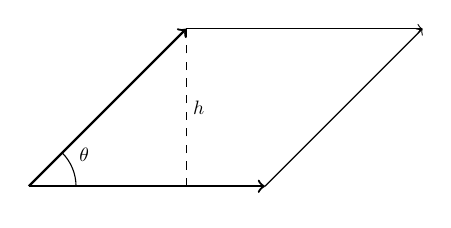
\begin{tikzpicture}[scale=1]
\draw[thick,->] (0,0) -- (3,0) node[pos=0.5, below,scale=0.7]{$\av$};
\draw[thick,->] (0,0) -- (2,2) node[pos=0.5, above left,scale=0.7]{$\bv$};
\draw[->] (3,0) -- (5,2) ;
\draw[->] (2,2) -- (5,2) ;
\draw[]  (0.6,0) arc (0:45:0.6) node[pos=0.5, above right, scale=0.7]{$\theta$};
\draw[dashed] (2,0) -- (2,2) node[pos=0.5, right,scale=0.7]{$h$};
\end{tikzpicture}
\end{center}



In $\FR^3$, on the other hand, three vectors $\av, \bv, \cv$ generically define a parallelepiped, as shown below. If one of the vectors is linearly dependent on the other two in will be coplanar with them and the parallelepiped will collapse to have zero volume. It is harder to picture in higher dimensions, but the idea is the same.

\begin{center}
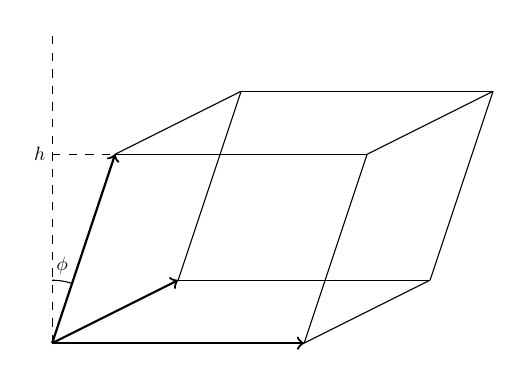
\begin{tikzpicture}[scale=0.8]
\draw[thick,->] (0,0) -- (1,3) node[pos=0.5, below right,scale=0.7]{$\av$};
\draw[thick,->] (0,0) -- (4,0) node[pos=0.5, below,scale=0.7]{$\bv$};
\draw[thick,->] (0,0) -- (2,1) node[pos=0.5, above left,scale=0.7]{$\cv$};
\draw[-] (4,0) -- (6,1) ;
\draw[-] (2,1) -- (6,1) ;

\draw[-] (1,3) -- (5,3) ;
\draw[-] (1,3) -- (3,4) ;
\draw[-] (5,3) -- (7,4) ;
\draw[-] (3,4) -- (7,4) ;

\draw[-] (4,0) -- (5,3) ;
\draw[-] (2,1) -- (3,4) ;
\draw[-] (6,1) -- (7,4) ;

\draw[dashed] (0,0) -- (0,5);
\draw[dashed] (0,3) -- (1,3) node [pos=0, left,scale=0.7]{$h$};
\draw[]  (0,1) arc (90:71.56:1) node[pos=0.5, above, scale=0.7]{$\phi$};
\end{tikzpicture}
\end{center}



\begin{example}{}
Using a determinant to test for a basis of $\FR^3$:


Let
\[
\vv_1=\begin{pmatrix}1\\0\\2\end{pmatrix},\qquad
\vv_2=\begin{pmatrix}0\\1\\-1\end{pmatrix},\qquad
\vv_3=\begin{pmatrix}3\\2\\1\end{pmatrix}.
\]
Form the associated matrix with these vectors as columns:
\[
A:=\left(\begin{array}{c|c|c}
\vv_1 & \vv_2 & \vv_3
\end{array}\right)
=
\begin{pmatrix}
1 & 0 & 3\\
0 & 1 & 2\\
2 & -1 & 1
\end{pmatrix}.
\]
Compute its determinant (expand along the first row, for example):
\[
\det(A)
=
1\cdot
\det\begin{pmatrix}1&2\\-1&1\end{pmatrix}
-0\cdot(\cdots)
+3\cdot
\det\begin{pmatrix}0&1\\2&-1\end{pmatrix}.
\]
Hence
\[
\det(A)
=
\bigl(1\cdot 1 - 2\cdot(-1)\bigr)
+3\bigl(0\cdot(-1)-1\cdot 2\bigr)
=
(1+2)+3( -2)
=
3-6
=
-3\neq 0.
\]
Therefore, by the theorem,
\[
\vv_1,\vv_2,\vv_3 \text{ is a basis of } \FR^3.
\]
\end{example}

We can also use the determinant test  when the vectors do {\it not} form a basis:

\begin{example}{}
Using a determinant to test for a basis of $\FR^3$ (an example where the vectors don't form a basis).

Let
\[
\vv_1=\begin{pmatrix}1\\0\\2\end{pmatrix},\qquad
\vv_2=\begin{pmatrix}0\\1\\-1\end{pmatrix},\qquad
\vv_3=\begin{pmatrix}1\\1\\1\end{pmatrix}.
\]
(Notice that \(\vv_3=\vv_1+\vv_2\).)

Form the associated matrix with these vectors as columns:
\[
A:=\left(\begin{array}{c|c|c}
\vv_1 & \vv_2 & \vv_3
\end{array}\right)
=
\begin{pmatrix}
1 & 0 & 1\\
0 & 1 & 1\\
2 & -1 & 1
\end{pmatrix}.
\]
Compute its determinant (expand along the first row, for example):
\[
\det(A)
=
1\cdot
\det\begin{pmatrix}1&1\\-1&1\end{pmatrix}
-0\cdot(\cdots)
+1\cdot
\det\begin{pmatrix}0&1\\2&-1\end{pmatrix}.
\]
Hence
\[
\det(A)
=
\bigl(1\cdot 1 - 1\cdot(-1)\bigr)
+\bigl(0\cdot(-1)-1\cdot 2\bigr)
=
(1+1)+(-2)
=
0.
\]
Therefore, by the theorem,
\[
\vv_1,\vv_2,\vv_3 \text{ do not form a basis of } \FR^3.
\]
(In fact they are linearly dependent since \(\vv_3=\vv_1+\vv_2\).)

\end{example}

